\section{Data integration and Interoperability}
\large \textbf{Apache Kafka}\\
\normalsize
\textbf{Connectors to external system}\\
Kafka provides the Kafka Connect framework to import data from external data systems to Kafka and export records from Kafka topics to sink storage systems \cite{kafkaconnect}. By using this framework, connectors for data integration can be quickly developed, deployed, and run in a scalable and fault tolerant way. 

Kafka Connect provides a uniform and high-level Java programming interface to develop connectors. Once the executable connector is built, it can be deployed to a Kafka Connect cluster. The Kafka Connect framework provides a REST API to deploy and manage connectors on the cluster. A Kafka Connect cluster runs independently from Kafka cluster and can comprise of multiple worker nodes. The tasks of copying data defined in the implementation of the connector can be distributed among these nodes for scalability. 

\begin{figure}[h]
	\centering
	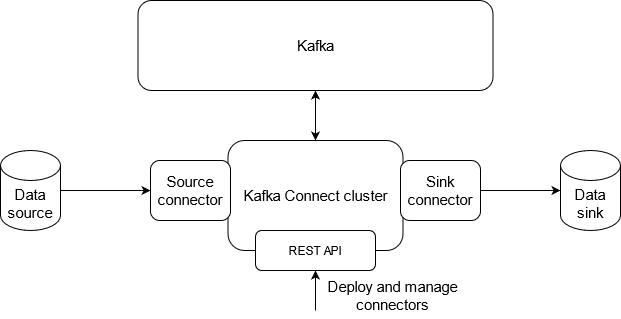
\includegraphics[width=10cm,height=6cm]{images/connector-kafka.png}
	\caption{Kafka Connect cluster to integrate data between Kafka and external data systems.}
	\label{fig:connectkafka}
\end{figure}

Internally, the workers in the connect cluster use Kafka clients to publish or consume data from Kafka. These worker coordinate with each other using the same balancing and failover mechanism as the Kafka consumer group. The framework automatically and periodically checkpoints the current processing positions on the source system of the copying task in Kafka. Developers do not have to take care of managing the consumption status of connector.

For the source connector which imports data into Kafka, the auto-management of consumption status cannot provide exactly-once guarantee in case of failure. This is because the framework does not use transactional feature of Kafka producer to save processing position along with the imported records \cite{kafkaconnectsource}. Therefore, if a worker node crashes before it checkpoints the consumption status on source system to Kafka, it is possible that some records will be reprocessed again when the copying task is resumed. 

With the sink connector which exports data from Kafka, users have the possibility to flush the offset number of the currently consumed record on the Kafka topic along with the actual data in a single atomic action to external data systems. Therefore, when worker node fails, the task can be resumed with the committed offset number on the external system instead of using the checkpointed position on Kafka. As a result, exactly-once semantics can be guaranteed on the sink system. For example, the sink connector to export data from Kafka to HDFS uses this approach to guarantee exactly-once semantics \cite{kafkahdfsconnector}.


With Kafka connector, users can also define a chain of simple and pluggable transformation operations to modify the records one after the other before they are written to destination systems \cite{kafkaconnect}. This can serve as a quick preliminary adaption of records so that they can match with the processing logic in their destination.

There are already many off-the-shelf connectors available for various data systems. The Confluent Hub, which is managed by the Confluent company, is a central repository to share Kafka connectors with both open-sourced and commercial licenses. There are connectors of many common data systems such as relational database, Hadoop distributed file system (HDFS), Cassandra, change data capture (CDC) on the source system. All these connectors can be quickly configured and deployed to a Kafka Connect cluster without any implementation requires. This can further offload the development burden on users to integrate Kafka with other data systems.



\textbf{Supported programming languages for clients}\\
The official release of Kafka includes only the Java client \cite{kafkaclients}. Kafka relies on different smaller groups of developers for providing clients in different programming languages. There are many third-party projects with more than 15 different supported programming languages such as C/C++, Python, Go. Most of these projects are very active and regularly updated along with the new release from Kafka.  

\large \textbf{Apache Pulsar}\\
\normalsize
\textbf{Connectors to external system}\\
Pulsar supports the automation of moving data in and out of Pulsar with the Pulsar IO connectors \cite{pulsario}. The concept of Pulsar IO is similar to Pulsar Functions. Developers can implement connectors using a Java programming interface provided by Pulsar. 

The executable files of connectors can then be deployed to the cluster of function workers on the Pulsar cluster using the REST API of the cluster or the admin command line tool of Pulsar. The connector is then run and scaled among the nodes of the function workers. 
Internally, Pulsar IO also uses normal Pulsar producer and consumer to interact with the Pulsar cluster. However, unlike the Kafka Connect framework, the management of reading position on the source system is not done transparently to users by Pulsar IO. Developers must handle the task of checkpointing the current consumption status of a connector and retrieving it when the connector is restarted. Therefore, the delivery semantics of a connector depends on the developers and which mechanism they use to commit the reading position. With the newly released Pulsar transaction, developers can utilize this feature to achieve exactly-once semantics for the connector. For instance, transaction is used in the implementation of sink connector to export data from Pulsar to Fink \cite{pulsarflinkconnector}.

In the official release of Pulsar, there are many ready-to-be-used source- and sink-connectors for different data systems such as relational databases, Kafka, HDFS, NoSQL databases. Users can simply start these connectors on the Pulsar cluster without having to download and deploy these connectors manually. There are also many other connectors developed and maintained by third-party organizations. For instance, Streamnative, which is a company offering managed Pulsar as a service, has a central hub with many Pulsar connectors.  

\textbf{Supported programming languages for clients}\\
Officially Apache Pulsar supports 7 different clients in different programming languages including some most popular languages such as Java, Python, and Node.js \cite{pulsarclients}.  Moreover, there are also other clients in 4 different languages all of which are actively maintained by third-party contributors. 

\large \textbf{NATS Streaming}\\
\normalsize
\textbf{Connectors to external system}\\
Currently there is not any general framework to move data in and out of NATS Streaming servers. There are only a few other projects which bridge NATS Streaming with some specific data systems such as Kafka and IBM-MQ \cite{natsclientsconnectors}. Moreover, these off-the-shelf connectors have to be deployed, managed and scaled manually by users. Other than that, if users want to connect NATS Streaming with external data systems, they need to handle the task of implementing, deploying and operating the connectors themselves. Therefore, integrating data with other systems is generally not supported by NATS Streaming. 

\textbf{Supported programming languages for clients}\\
Syndia, which is the company actively develops and maintains the NATS Streaming project, officially supports clients in 7 different programming languages with some common languages: Java, C, Node.js \cite{natsclientsconnectors}. In addition, there are some other clients maintained by the community. Nevertheless, these projects are very inactive and outdated. Therefore, these third-party clients will not be included in the evaluation.      
